\begin{multicols*}{2}
    
\section{Project proposal}

This project is part of the \href{https://membres-ljk.imag.fr/Christophe.Picard/teaching/gp-gpu}{GP-GPU Computing course} at UGA by Christophe Picard. Here, we present a proposal for the final project.

The \gls{ipa} uses special symbols\footnote{See for example the French list \href{https://en.wikipedia.org/wiki/Help:IPA/French}{here}.} to represent the sound of a spoken language. Especially in French, the pronunciation of words can be quite different from the written form, which is why the phonetic alphabet is useful. For new language learners and phonetic enthusiasts alike it could be interesting to find groups of words that sound familiar to a given word. Identifying such groups helps setting a word in a broader context and thus remembering it, and also fosters a joyful play with language.

In order to evaluate the closeness of two words, we need to \textbf{define a metric that quantifies the distance of two words}. We only consider their phonetic transcription, \ie homophones like the French words \q{vert} (green) and \q{verre} (glass) have a distance of 0 and are considered the same (in the phonetic sense). For the distance metric, we will employ the \textbf{Needleman-Wunsch algorithm}, which calculates the global alignment of two sequences and was originally used in bio-informatics to compare DNA sequences. Here, the alphabet will instead consist of the phonetic symbols. Out of all possible alignments of two words (including gaps), the Needleman-Wunsch algorithm finds the one with the smallest distance, \ie the alignment with the highest score. A good introduction to the algorithm can be found on the respective \href{https://en.wikipedia.org/wiki/Needleman%E2%80%93Wunsch_algorithm}{Wikipedia page}.

To evaluate the feasibility of this project, we combined different datasets to create a new one consisting of \textbf{700,000 French words and their phonetic transcription} as well as their frequency in the French language\footnote{In the final report, we will provide more details on the dataset and their sources.}. We implemented a Rust program that calculates the distance of all pairs of words. This corresponds to \textbf{computing the weights for all edges of a fully-connected graph}, where nodes are the words (their phonetic transcriptions) and edges have weights corresponding to the distance between the words. For the full dataset, we thus find:

\begin{align}
    \text{Number of nodes} &= 700,000 \\
    \text{Number of edges} &= \frac{1}{2} \cdot 700,000 \cdot 699,999 \\
    &=  244,999,650,000
\end{align}
This presents a huge challenge both to computation and memory. Even if we only stored each edge weight with 7~bits, the edges alone would require $\approx \qty{214}{\giga\byte}$ of memory. With regards to computation, the algorithms lends itself to parallelization, as the distance calculation of two words is independent of other word pairs.

After a first Python implementation, we wrote a Rust program to calculate the distance with Needleman-Wunsch. It was parallelized on a 4-core consumer CPU using the Rayon library. Based on calculations on the first 20,000 words, we estimate that the implementation will take $\approx \qty{3}{\hour}$ to calculate the distances for all word pairs. This could be acceptable as it only has to be done once. After that, the lookup is in $\mathcal{O}(1)$ time.

However, we also want to adopt a \textbf{custom scoring matrix} for the Needleman-Wunsch algorithm that takes into account phonetic symbol similarity itself. For example, replacing a \textit{b} by a \textit{p} should have a lower penalty than replacing a \textit{b} by an \textit{m}. Defining such a matrix a priori based on random word pairs where only one sound is changed (minimal pairs) has turned out to be difficult. A better approach could be to calculate all distances with a given default scoring (1 on the diagonal, -1 on off-diagonals), then use the results to get the neighbors of a word. With this, we get a better understanding of what words are considered similar by the algorithm and can adjust the scoring matrix accordingly. This iterative process requires a fast implementation of the Needleman-Wunsch algorithm to reduce the turnaround time.

Future works could discuss how clustering algorithms like the Louvain method can be parallelized in a way that also allows only reading parts of the dataset at a time. By doing so, we could cluster words based on their phonetic similarity and thus find \textit{groups of words} that sound similar (compared to only finding the neighbors of a word).

\end{multicols*}


\begin{figure}[ht]
    \centering
    \subfigure[Neighbors of \q{glace}]{
        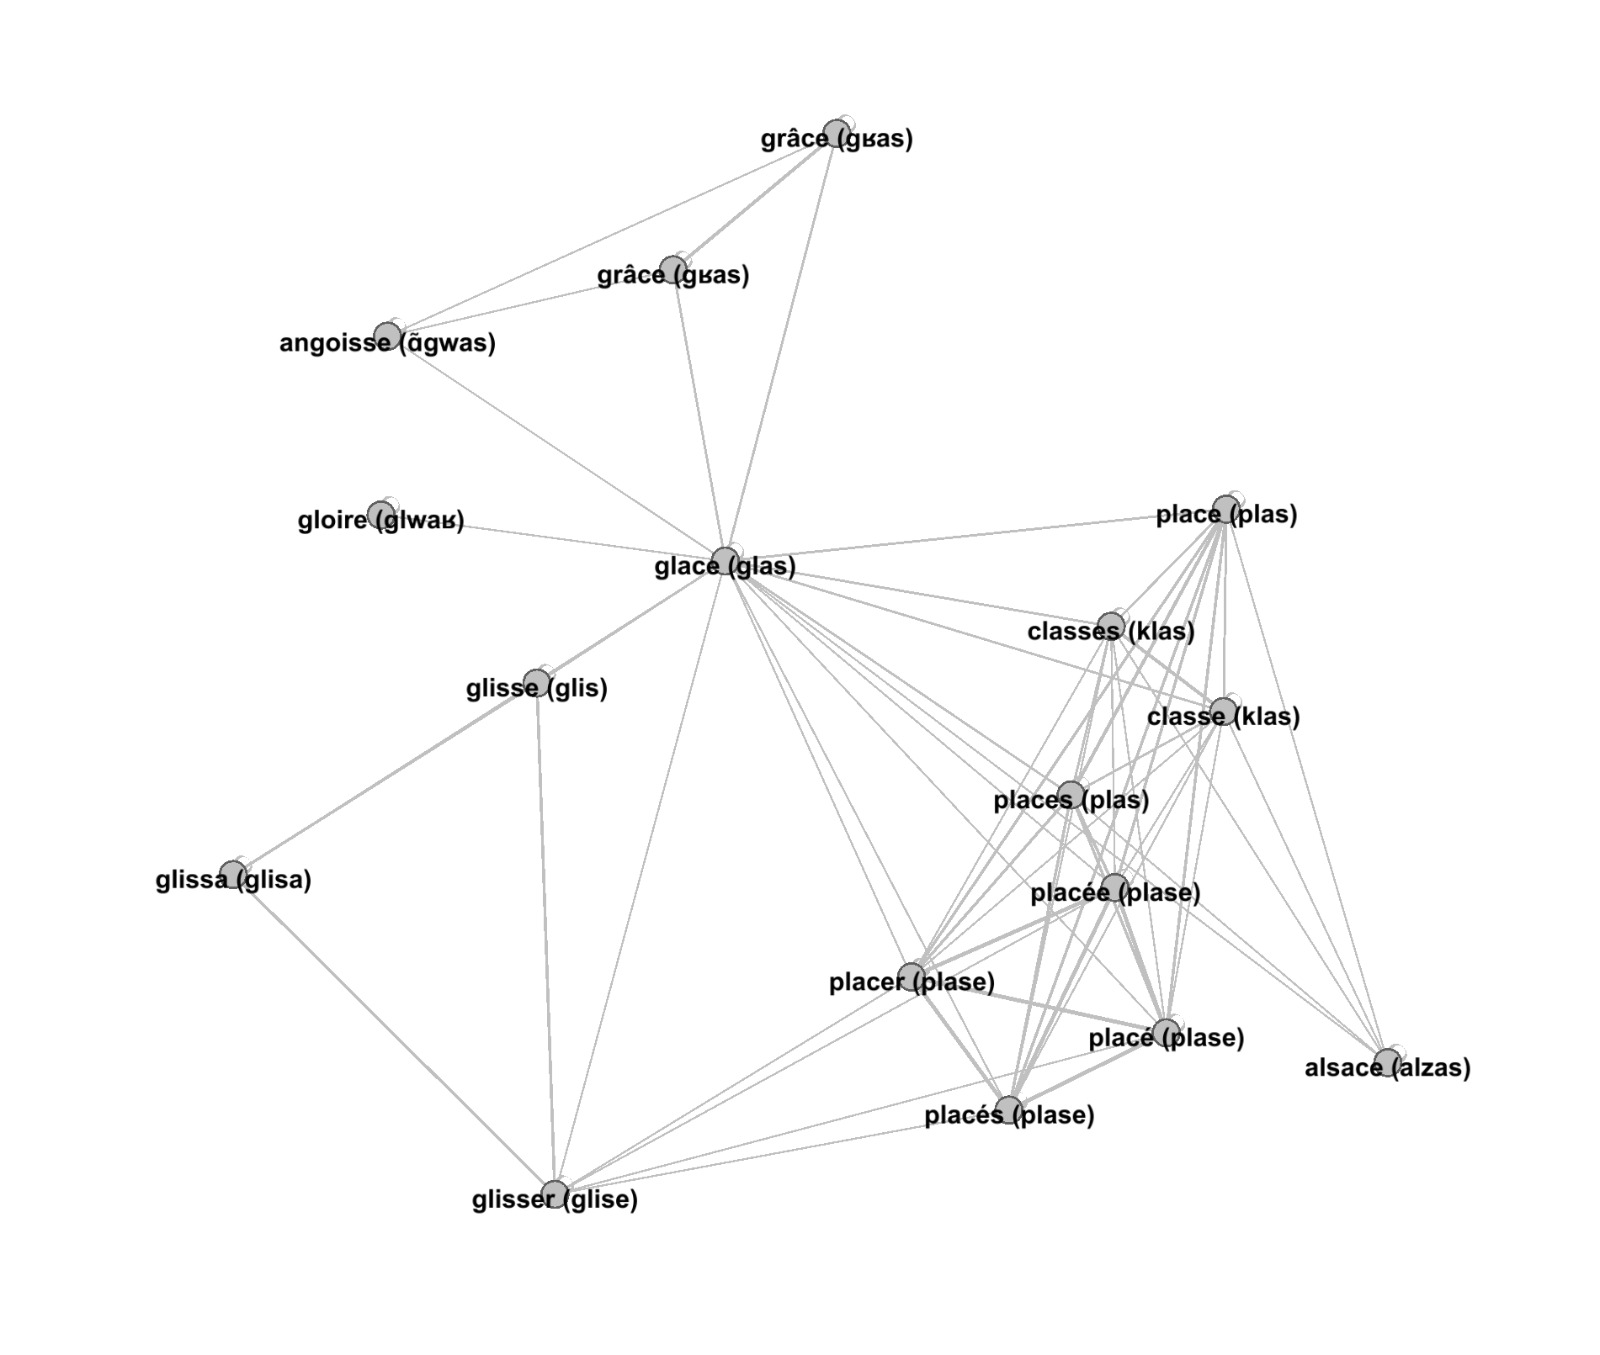
\includegraphics[width=0.45\textwidth,trim={5cm 4cm 4cm 4cm},clip]
            {assets/glace-neighbors.jpeg}
    }
    \hfill
    \subfigure[Neighbors of \q{prévoir}]{
        \includegraphics[width=0.45\textwidth,trim={3.5cm 3.5cm 4cm 3.5cm},clip]
            {assets/prévoir-neighbors.jpeg}
    }
    \caption{Visualization of neighbors based on phonetic distance. Edge weights encode the closeness of two words. Colors are artifacts of a previous visualization and can be ignored.}
    \label{fig:neighbors}
\end{figure}

\begin{multicols*}{2}


Based on the first 10,000 most frequently used words, we calculated the distance between every pair and visualized the graph using \href{https://gephi.org/}{Gephi's} ForceAtlas2 algorithm. The neighbors of the word \q{glace} and \q{prévoir} are shown in \autoref{fig:neighbors}. For bigger graphs than that, Gephi is not able to handle the amount of data anymore.

Having translated the problem into a graph structure also allows us to use graph algorithms to discover interesting properties. As an example, Gephi implements the \textit{shortest path algorithm}: users can click on two words and the shortest path between them is calculated and shown in the graph. Beforehand, we filtered the graph to only include the most strong edges. With this, we can find chains like the following (read them aloud to hear the phonetic similarity):
\begin{itemize}
    \item trottoir $\rightarrow$ entrevoir $\rightarrow$ devoir $\rightarrow$ voire $\rightarrow$ voile $\rightarrow$ val $\rightarrow$ valait $\rightarrow$ fallait $\rightarrow$ falaise
    \item falaise $\rightarrow$ fallait $\rightarrow$ palais $\rightarrow$ passais $\rightarrow$ dépassait $\rightarrow$ dépendait $\rightarrow$ répondait $\rightarrow$ répond $\rightarrow$ raison $\rightarrow$ maison
    \item confusion $\rightarrow$ conclusion $\rightarrow$ exclusion $\rightarrow$ explosion $\rightarrow$ exposition $\rightarrow$ explications $\rightarrow$ respiration $\rightarrow$ précipitation $\rightarrow$ présentation $\rightarrow$ présenta $\rightarrow$ présente $\rightarrow$ présence $\rightarrow$ présidence $\rightarrow$ résidence $\rightarrow$ résistance $\rightarrow$ existence
\end{itemize}

\printglossary[type=\acronymtype]

\end{multicols*}

\begin{algorithm}
    \DontPrintSemicolon
    
    \SetKwFunction{FRandomCommunityMutation}{randomCommunityMutation}
    \SetKwFunction{FMutateRandomly}{mutateRandomly}
    \SetKwFunction{FgetRandomVertices}{getRandomVertices}
    \SetKwFunction{FDrawUniformly}{drawUniformly}
    
    \KwIn{$numVertices \!: \text{int}$}
    \Fn{\FgetRandomVertices{}}
    {
        \label{alg:mutate-random:getRandomVertices}
        $vertices \gets \emptyset$\;
        \While{$|vertices| \neq numVertices$}
        {
            \label{alg:mutate-random:fill-vertices-set-in-get-random}
            $vertices \gets vertices \: \cup $ \FDrawUniformly{$[0,n)$}\;\label{alg:mutate-random:fill-set}
        }
        \Return $vertices$\;
    }

    \BlankLine
    \BlankLine
    \BlankLine

    \Fn{\FRandomCommunityMutation{}}
    {
        $numNodesMutate \gets$ \FDrawUniformly{$[1, 0.1n]$}\;\label{alg:mutation-random:numNodesMutate}
        $randomVertices \gets$ \FgetRandomVertices{$numNodesMutate$}\;
        \ForEach{Vertices $v \in randomVertices$}
        {
            \FMutateRandomly{v}\;	
        }
    }

    \BlankLine
    \BlankLine
    \BlankLine

    \KwIn{$v \! : \text{Vertex to mutate}$}
    \Fn{\FMutateRandomly{}}
    {
        $c_v \gets $ \FDrawUniformly{$[0,2\cdot |fittestChromosomeCommunities|]-1$}\;\label{alg:mutation-random:assign-community}
    }
    
    \caption{Random community mutation}
    \label{alg:mutation-random}
\end{algorithm}
